%%% Template originaly created by Karol Kozioł (mail@karol-koziol.net) and modified for ShareLaTeX use

\documentclass[addpoints]{exam}

\usepackage[T1]{fontenc}
\usepackage[utf8]{inputenc}
\usepackage{graphicx}
\usepackage{xcolor}

\renewcommand\familydefault{\sfdefault}
\renewcommand{\theenumi}{\Alph{enumi}}
\usepackage{tgheros}

\usepackage{amsmath}
\usepackage{amssymb,amsthm,textcomp}
\usepackage{enumerate}
\usepackage{multicol}
\usepackage{tikz}
\usepackage[spanish, es-nodecimaldot]{babel}
\usepackage{enumitem}


\usepackage{geometry}
\geometry{left=25mm,right=25mm,bindingoffset=0mm, top=20mm,bottom=20mm}


\linespread{1.3}

\newcommand{\linia}{\rule{\linewidth}{0.5pt}}

% custom theorems if needed
\newtheoremstyle{mytheor}
{1ex}{1ex}{\normalfont}{0pt}{\scshape}{.}{1ex}
{{\thmname{#1 }}{\thmnumber{#2}}{\thmnote{ (#3)}}}
  
  \theoremstyle{mytheor}
  \newtheorem{defi}{Definition}
  
  % my own titles
  \makeatletter
  \renewcommand{\maketitle}{
    \begin{center}
    \vspace{2ex}
    {\huge \textsc{\@title}}
    \vspace{1ex}
    \\
    \linia\\
    \@author \hfill \@date
    \vspace{4ex}
    \end{center}
  }
  \makeatother
  %%%
  
  % custom footers and headers
  %\usepackage{fancyhdr}
  %\pagestyle{fancy}
  \lfoot{Parcial \textnumero{} 2}
  \cfoot{}
  \rfoot{Page \thepage}
  %\renewcommand{\headrulewidth}{0pt}
  %\renewcommand{\footrulewidth}{0pt}
  
  % code listing settings
  \usepackage{listings}
  \lstset{
    language=Python,
    basicstyle=\ttfamily\small,
    aboveskip={1.0\baselineskip},
    belowskip={1.0\baselineskip},
    columns=fixed,
    extendedchars=true,
    breaklines=true,
    tabsize=4,
    prebreak=\raisebox{0ex}[0ex][0ex]{\ensuremath{\hookleftarrow}},
    frame=lines,
    showtabs=false,
    showspaces=false,
    showstringspaces=false,
    keywordstyle=\color[rgb]{0.627,0.126,0.941},
    commentstyle=\color[rgb]{0.133,0.545,0.133},
    stringstyle=\color[rgb]{01,0,0},
    numbers=left,
    numberstyle=\small,
    stepnumber=1,
    numbersep=10pt,
    captionpos=t,
    escapeinside={\%*}{*)}
  }
  %%%----------%%%----------%%%----------%%%----------%%%
  
  %%%----------%%%----------%%%----------%%%----------%%%
  
  \begin{document}
  
  \title{Parcial 1 - Estadística I}
  
  \author{ITAM, Otoño 2022}
  
  \date{14/11/2022}
  
  \maketitle
  
  \section*{Instrucciones}
  
El examen tiene una duración de 1:40 horas y comienza a las 20:00 hrs. Se debe cuidar la formalidad al escribir los resultados, ya que es parte de la calificación del problema. En caso de no tener el desarrollo de la pregunta, o bien se llegué a la respuesta sin una justificación se podrá anular la respuesta. \textbf{Cualquier práctica fraudulenta será sancionada de acuerdo al reglamento.} 

\vspace{10pt}
  
  \section*{Seccion A: Preguntas a desarrollar (23 pts)}
  
  \begin{questions} 
  
  \question (4 pts) 
  Los Pumas de la UNAM y los Rayados de Monterrey organizan una competencia entre ellos dos para ver cuál es mejor equipo. El primero que gane dos juegos ganará la competencia, considere que ganar un partido es independiente de los demás. En un portal de apuestas se tiene que la probabilidad que los Pumas le ganen a los rayados es de 0.6 por partido, además en cada juego debe haber un solo ganador (sin empates). Adiccional a esto, los partidos impares 1,3,5,7,... se juegan en el Estadio de CU y los partidos pares 2,4,6,8,... en el Estadio BBVA. Resuelva los siguientes incisos:
  \begin{enumerate}[label=\Alph*)]
  \item (0.8 pts) Calcule la probabilidad que los pumas ganen la competencia
  \item (0.8 pts) Calcule la probabilidad que solo se jueguen dos partidos
  \item (0.8 pts) Calcule la probabilidad que el último partido de la competencia sea en el estadio de CU
  \item (0.8 pts) Calcule la probabilidad que los pumas ganen su segundo partido en el estadio BBVA
  \item (0.8 pts) Calcule la probabilidad que dado que los pumas gane el primer partido de la competencia, gane el segundo partido de la competencia
  \end{enumerate}
  
\question (3 pts)
Para pasar el examen final de estadística 1 los alumnos del ITAM tienen solo dos opciones para estudiar. El método A es ir a todas las clases con su profesor y hacer todos los ejercicios del cuadernillo, mientras que el método B es ver los videos del Julio profe (solo pueden elegir uno de estos dos métodos). El porcentaje de alumnos reprobados en el método A es 20\% y el porcentaje de alumnos reprobados por el método B es de 50\%. Se sabe que el 80\% de los alumnos de estadística cumplen cabalmente con el método A. 
\begin{enumerate}[label=\Alph*)]
\item (1.5 pts) Dado que un alumno aprobó, cual es la probabilidad que haya estudiado con el método B
\item (1.5 pts) Dado que un alumno reprobó, cual es la probabilidad que haya estudiado con el método A
\end{enumerate}

\question (4 pts)
En una empresa de crean 2 posiciones nuevas a las que aspiran 8 personas. De esas 8 personas 3 pertenecen al área de Sistemas, 3 al área de Ventas y 2 al área de Estrategia Comercial. Se sabe que los 8 aspirantes tienen la misma probabilidad de ser seleccionados, por lo que sea X la variable que indica el número de personas seleccionadas que provienen de sistemas, Y el número seleccionadas de personas que provienen del área de ventas.
\begin{enumerate}[label=\Alph*)]
\item (1 pts) Construya la tabla de probabilidad conjunta de X y Y
\item (1 pts) Encuentre las distribuciones marginales de X y Y
\item (1 pts) ¿Cuál es el valor esperado y varianza de X y Y?
\item (1 pts) Si Z es el número de personas que pertenecen al área de estrategia comercial, obtenga su valor esperado y varianza
\end{enumerate}
 
\question (4 pts) Un proveedor de maquinaria para construcción ha encontrado que la probabilidad de venta de una pieza por medio de una llamada es de 0.3, la probabilidad de venta es independiente entre llamadas. Si el proveedor tiene 3 máquinas, ¿Cuál es la probabilidad que se requieran menos de 5 llamadas para vender todas las máquinas?
  
 
\question (4 pts) El número de colonias de bacterias en agua contaminada se distribuye Poisson con una media de 2 por $cm^3$
\begin{enumerate}[label=\Alph*)]
\item (2 pts) Si cuatro muestras de 1 $cm^3$ se seleccionan de esta agua de manera independiente, encuentre la probabilidad de que al menos una muestra contenga una o más colonias de bacterias
\item (2 pts) ¿Cuántas muestras de 1 $cm^3$ deben seleccionarse para tener una probabilidad de 0.98 de ver al menos una colonia de bacterias?
\end{enumerate}

\question (4 pts)  A veinte estudiantes se les pide seleccionar números enteros entre el 1 al 10.
\begin{enumerate}[label=\Alph*)]
\item (2 pts) ¿Cuál es la probabilidad que 8 o más estudiantes seleccionen los números 4,5 o 6?
\item (2 pts) Dado que se sabe que 5 o más estudiantes seleccionaron los números 4,5,6, ¿Cuál es la probabilidad que 8 o más estudiantes seleccionen los números 4,5,6?
\end{enumerate}

\newpage

Tabla Binomial

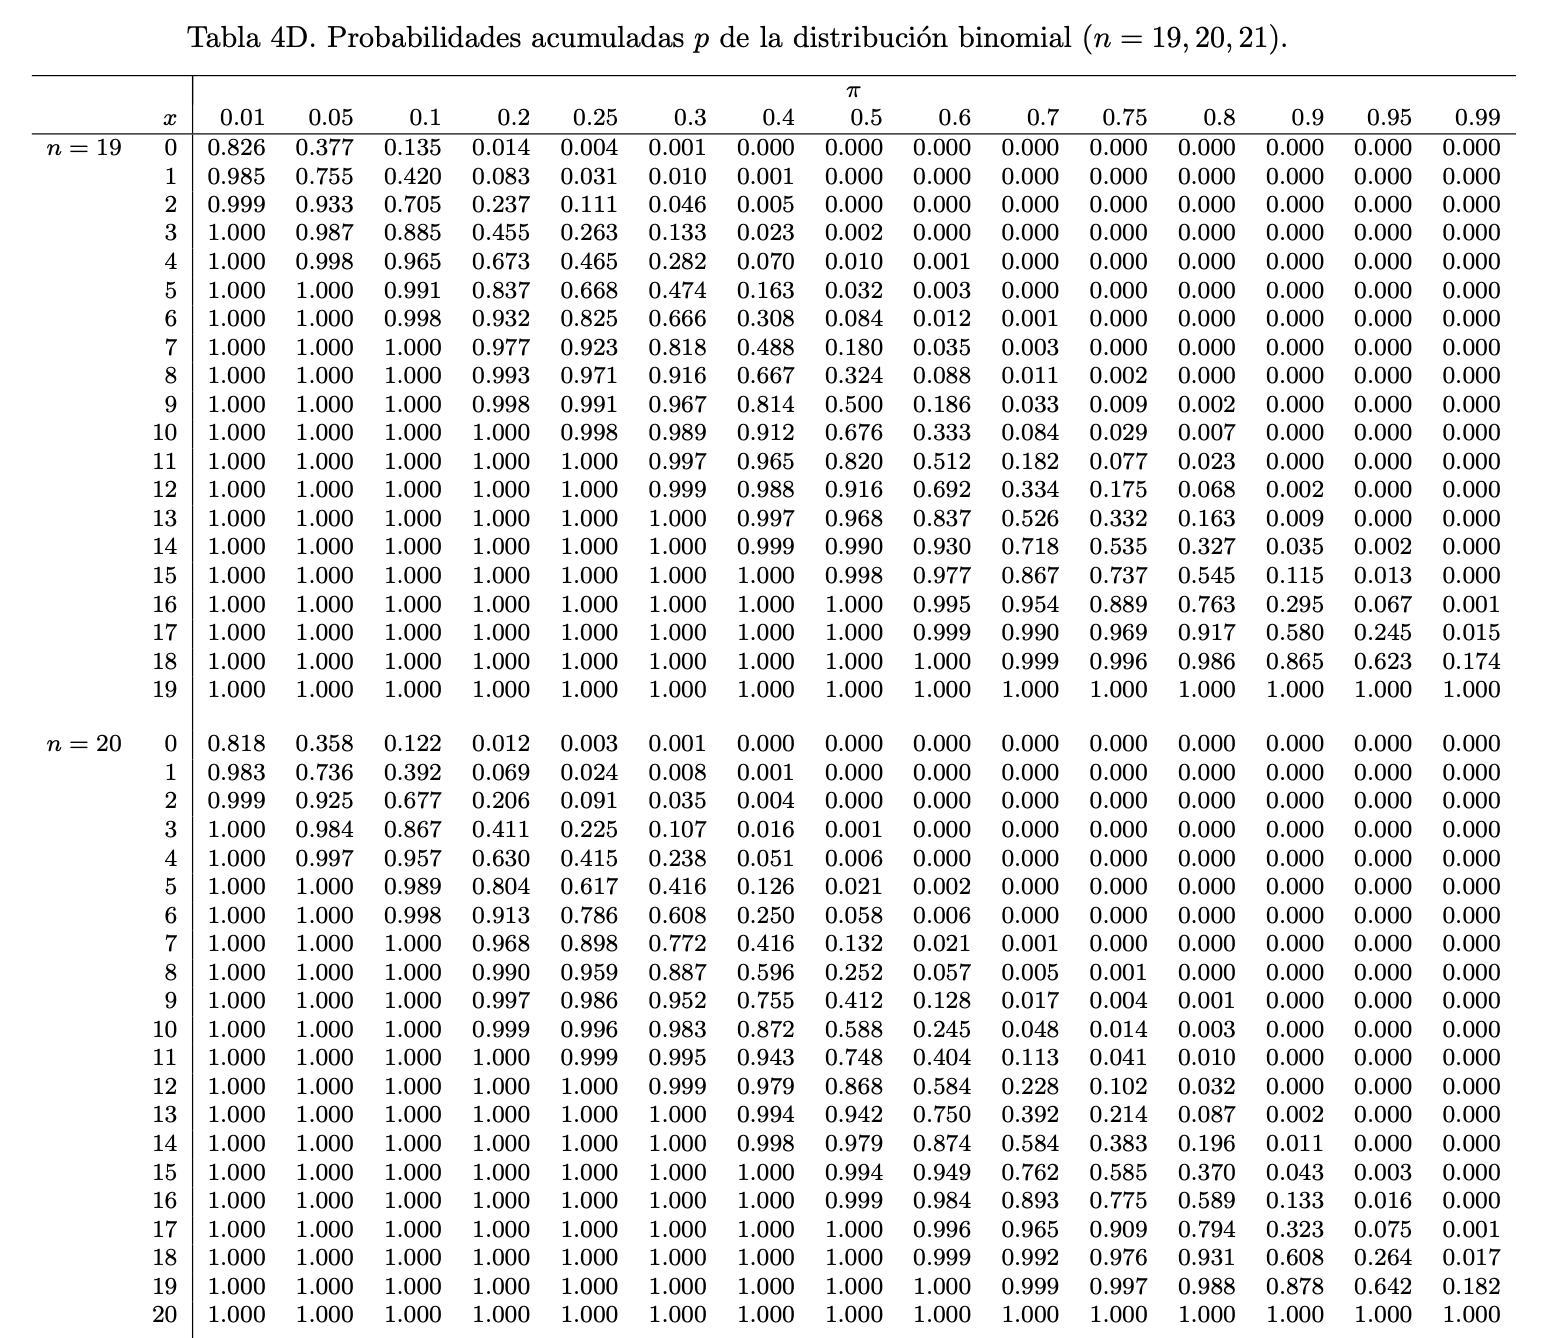
\includegraphics[width=15cm]{tabla_binomial.png}

\newpage
Tabla Poisson

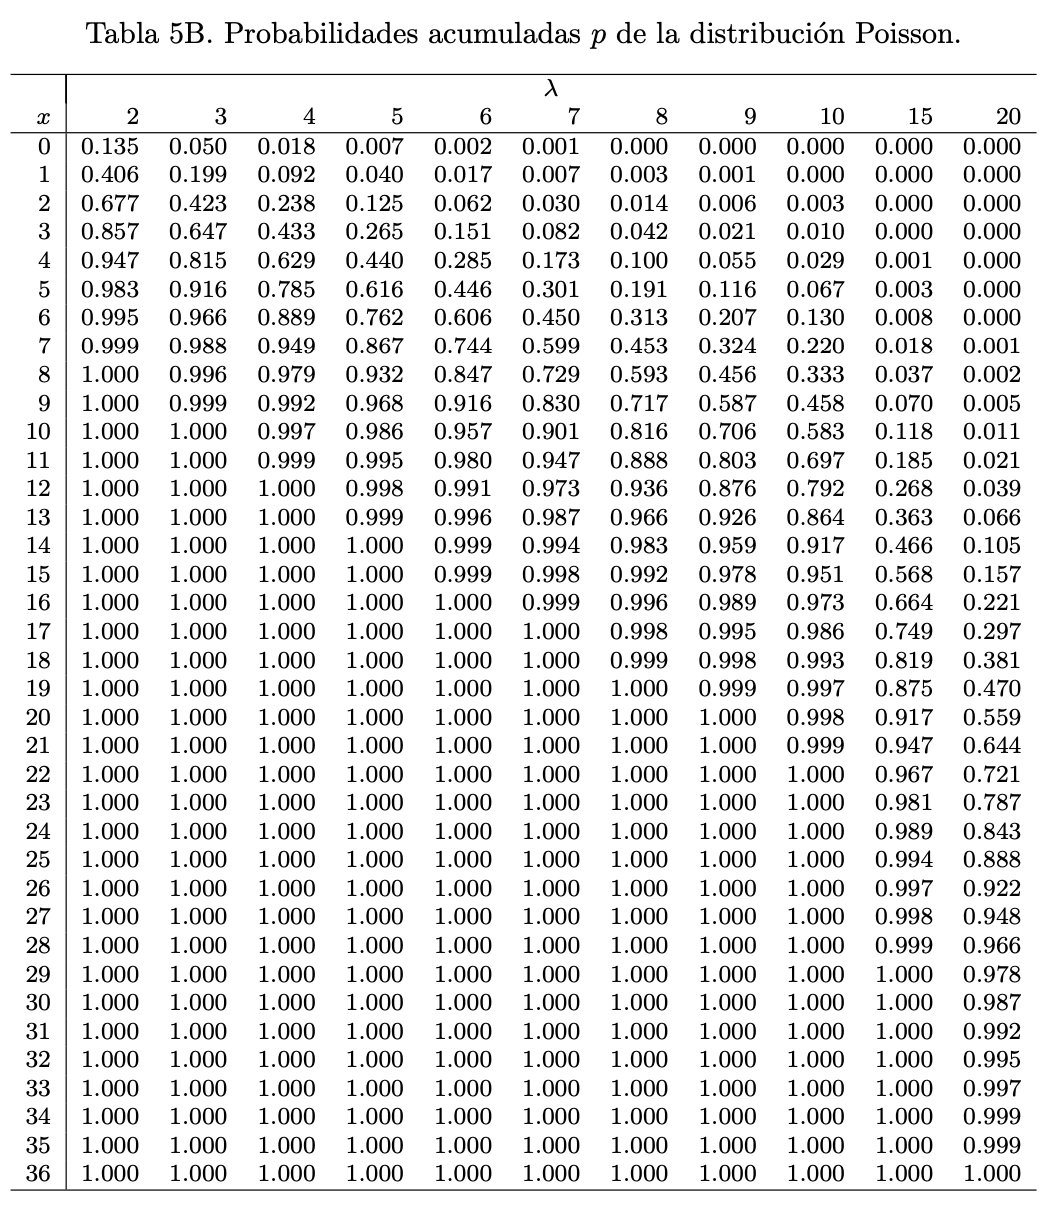
\includegraphics[width=15cm]{tabla_poisson.png}


\end{questions}

\end{document}
  

